\documentclass[letterpaper, conference]{IEEEtran}
\IEEEoverridecommandlockouts
% The preceding line is only needed to identify funding in the first footnote. If that is unneeded, please comment it out.
\usepackage{cite}
\usepackage{amsmath}
\usepackage{amssymb,amsfonts}
\usepackage{algorithmic}
\usepackage{graphicx}
\usepackage{textcomp}
\usepackage{xcolor}
\usepackage[utf8]{inputenc}
\usepackage{float}
\usepackage{subcaption}
\usepackage{minted}
\usepackage{xcolor}

\usemintedstyle{friendly}

\usepackage[pdftex]{hyperref}
\hypersetup{
	colorlinks=true,
	linkcolor=blue,
	filecolor=magenta,      
	urlcolor=blue,
	citecolor=blue,
	pdftitle={Pax Animi},
	pdfauthor={Daniel E. Hernández}
	bookmarks=true,
	bookmarksopen=true,
	pdfpagemode=FullScreen,
}



\makeatletter
\renewcommand*\env@matrix[1][*\c@MaxMatrixCols c]{%
	\hskip -\arraycolsep
	\let\@ifnextchar\new@ifnextchar
	\array{#1}}
\makeatother


\def\BibTeX{{\rm B\kern-.05em{\sc i\kern-.025em b}\kern-.08em
		T\kern-.1667em\lower.7ex\hbox{E}\kern-.125emX}}
\begin{document}
	
	\title{Demonstrations of Linear-Regressions in Python with Least Squares Method*\\
		\thanks{Thanks to Christiaan Ketelaar and Carlos Morales for their help on understanding linear algebra and its applications.}
	}
	
	\author{\IEEEauthorblockN{Daniel E. Hernández Zelada}
		\IEEEauthorblockA{\textit{Computer Science Student. (of FCE)} \\
			\textit{Universidad Francisco Marroquín}\\
			Guatemala, Guatemala \\
			\href{mailto:danielernesto@ufm.edu}{\texttt{danielernesto@ufm.edu}}}
}
	
	\maketitle
	
	\begin{abstract}
		This document is a demonstration of Linear-Regressions through python. It solves two problems with two subsets of problems one of which is optimizing the best-fitting function to find the maximum value possible given some real world restrictions.
	\end{abstract}
	
	\begin{IEEEkeywords}
		linear algebra, regression, optimizing, least squares
	\end{IEEEkeywords}
	
	\section{Introduction}
		This document explains the process of finding the least squares for linear-regressions on Python and using them ro predict data and maximize functions.
	
	\section{Least Squares}
		\subsection{Description of the Problem}
			Often in the world, one finds that particular data gathered through time--for example--can be related with a linear equation. 
			Least squares is a method of finding such linear equation through matrices constructed with data sets to build a best-fit function to approximate as accurately as possible to the real data. 
			
			These functions can be used to predict the behavior of events in the future. Though it's important to note that their precision will, of course, depend on the magnitude of the error.
			
		\subsection{Normal Equation}
			To initialize the construction of such system, one needs to be familiarized with the main equation used with the \textit{Least Squares} method, i.e. the \textit{Normal Equation} which is as follows.
			\begin{equation}
				A^T A \vec{x} = A^T \vec{b} \label{Normal Equation}
			\end{equation}
			Matrix A is composed of 1s in the first column while the second column is built  with $x_{1}$ (i.e. the independent variable(s)). Note: If the experiment had more than one $x$ e.g. from $x_{1}$ to $x_{n}$ it would still be constructed by the same principle, first column of 1s and the next columns would be the different independent variables. It can be of shape (m,n).
			
			The $\vec{b}$ on the other hand is constructed with de dependent variables, often $y$ it can only be of shape (m,1).
		\begin{figure}
			\centering
			\begin{subfigure}{.2\textwidth}
				\[
				\begin{bmatrix}
				1       & ax_{1}  & \dots & ex_{n} \\
				1       & bx_{1}  & \dots & fx_{n} \\
				1       & cx_{1}  & \dots & gx_{n} \\
				\vdots	& \vdots  & \vdots& \vdots \\
				1       & dx_{1}  & \dots & hx_{n} \\
				\end{bmatrix}
				\]
				\caption{Matrix A.}
				\label{figure1}
			\end{subfigure}
			\begin{subfigure}{.2\textwidth}
				\centering
				\[
				\begin{bmatrix}
				1       & 5  \\
				1       & 3  \\
				1       & 8  \\
				1	    & 7  \\
				1       & 10 \\
				\end{bmatrix}
				\]
				\caption{Matrix A.}
				\label{figure2}
			\end{subfigure}
		\end{figure}

		\begin{figure}[H]
			\centering
			\begin{subfigure}{.2\textwidth}
				\[
				\begin{bmatrix}
				4  \\
				5  \\
				5  \\
				5  \\
				6  \\
				\end{bmatrix}
				\]
				\caption{$\vec{b}$.}
				\label{figure3}
			\end{subfigure}
			\begin{subfigure}{.2\textwidth}
				\centering
				\[
				\begin{bmatrix}
				\frac{\sqrt{3}}{2}  \\
				\pi \\
				10.2 \\
				64	    \\
				8 \\
				\end{bmatrix}
				\]
				\caption{$\vec{b}$.}
				\label{figure4}
			\end{subfigure}
		\caption{Examples of A Matrices}
		\end{figure}
		
		\subsection{General Proceedings}
			After the equations have been completed, one needs to make an augmented matrix of the form:
			\begin{figure}[H]
				\centering
				\[
				\begin{bmatrix}[c|c ]
					A^T A & A^T \vec{b} \\
				\end{bmatrix}
				\]
				\caption{Augmented Matrix.}
				\label{figure5}
			\end{figure}
			Once Gauss-Jordan elimination has been done, the solutions of said augmented matrix will be $C_{0}$ which will be the intercept and $C_{1}$ which will be the slope of the linear-approximation function. So when one builds the function with the given coefficients it yields as follows:
			\begin{equation}
			y = C_{0} + C_{1}x \label{augmented equation}
			\end{equation}
		

		\section{Procedures for Exercise One}
			The first exercise was executed using two methods of the Least Squares algorithm. In the former, the column of 1s was added manually as seen on:
				\begin{center}
					\inputminted[
					firstline=26, 
					lastline=34,
					linenos,
					xleftmargin=20pt,
					breaklines, 
					breakautoindent=false,
					] {python}{../src/lab.py}
				\end{center}
			The more automated version is found on:
				\begin{center}
					\inputminted[
					firstline=104, 
					lastline=104,
					linenos,
					xleftmargin=20pt,
					breaklines, 
					breakautoindent=false,
					] {python}{../src/lab.py}
				\end{center}
			which is used in latter and in the second exercise; said method appends a second column of 1s but now at the right of the original numbers instead of the original formula which would have them on the left. The reason of doing so is because it's really just a prerequisite by the rest of NumPy's functions.
			
			The equation used on both methods is the Normal Equation (as seen on: \ref{Normal Equation}) and the proceedings followed the augmented matrix (as seen on: \ref{figure5}) which is necessary to be able to then get $C_{0}$'s and $C_{1}$'s values, though the second method solved the matrix through \texttt{m, b = np.linalg.lstsq(A, y, rcond=None)[0]} which automatically returns the coefficients in an array-like form which then can later be manipulated. 
			
			Then the linear-approximation function (\ref{augmented equation}) was built to predict, as the clause \textit{a)} asked, a new life expectancy estimate based on the last events for the year 2000.
			
			\subsection{Default Matrices}
					\begin{figure}[H]
						\centering
						\begin{subfigure}{.2\textwidth}
							\centering
							\[
							\begin{bmatrix}
							1 & 1920 \\
							1 & 1930 \\
							1 & 1940 \\
							1 & 1950 \\
							1 & 1960 \\
							1 & 1970 \\
							1 & 1980 \\
							1 & 1990 \\
							\end{bmatrix}
							\]
							\caption{Matrix A}
							\label{matrixA_1}
						\end{subfigure}
						\begin{subfigure}{.2\textwidth}
							\centering
							\[
							\begin{bmatrix}
							54.1 \\
							59.7 \\
							62.9 \\
							68.2 \\
							69.7 \\
							70.8 \\
							73.7 \\
							75.4 \\
							\end{bmatrix}
							\]
							\caption{$\vec{b}$.}
							\label{matrixb_1}
						\end{subfigure}
					\caption{Matrices extracted from Ex. One's data set}
					\end{figure}
			\subsection{Normal Equations}
			Following the normal equation (\ref{Normal Equation}) we get that $A^TA$ is as follows:
			\begin{figure}[H]
				\centering
				\[
				\centering
				\left[
				\begin{matrix}
				8 & 15640\\
				15640 & 30580400
				\end{matrix}
				\right]
				\]
				\caption{First part of the Normal Equation}
				\label{ATA_1}
			\end{figure}
			
			And we get $A^T\vec{b}$ as follows:
			\begin{figure}[H]
				\centering
				\[
				\centering
				\left[
				\begin{matrix}
				534.5\\
				1046169.0
				\end{matrix}
				\right]
				\]
				\caption{Second part of the Normal Equation}
				\label{ATb_1}
			\end{figure}
		 
		 We now construct the augmented matrix and solve it by using Gauss-Jordan elimination:
		 \begin{figure}[H]
			\centering
			\[
			\begin{bmatrix}[c c|c ]
				8 & 15640 		 &				534.5\\
				15640 & 30580400 &				1046169.0
			\end{bmatrix}
			\]
			\caption{Augmented Matrix.}
			\label{ATAB_1 Augemented}
		 \end{figure}
	 
	 Once solved we get that $C_{0}=-501.77$ and 
	 $C_{1}=0.29083$. Thus constructing the best-fit linear approximation of:
	 \begin{equation}
	 	y = -501.767 + 0.291x
	 	\label{Exercise One Final Equation}
	 \end{equation}
	 Now that we have the final function we can make a reasonably well prediction of the life expectancy of the year 2000. Given that the years are the independent variable we just do $f(2000)= -501.767 + 0.291(2000)$ which results in: 79.9 years.
	 
	\subsection{Graph and Precision Analysis}
	\begin{figure}[H]
		\centering 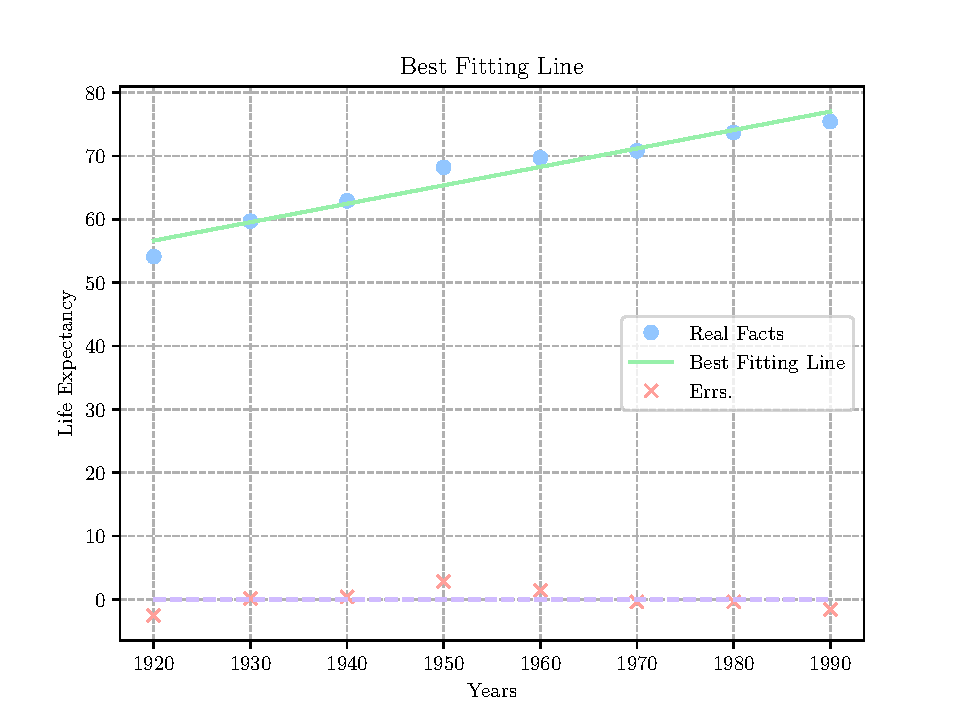
\includegraphics[scale=0.5]{../Graph_1.pdf}
		\caption{Life expectancy in relation to decades and errors.}
		\label{image1}
	\end{figure}
	
	Given that the linear approximation fits sufficiently well with the data given, it is reasonable to conclude that this model is safe for making short-term predictions.
	
	\section{Procedures for Exercise Two}
	The second exercise was built using only the automated method mentioned in the last procedures. However the data set was not `hard-coded' but depends on an external file, an Excel file. 
	
	This exercise prompts the user for the file destination through the standard OS GUI for file exploring. Upon selecting the designated Excel file, the program loads the data frame into an array in the memory. Given that said array is of shape (22,2), the program extracts each side of the original array into two (22,1) numpy matrices as seen on:
	\begin{center}
		\inputminted[
		firstline=148, 
		lastline=152,
		linenos,
		xleftmargin=20pt,
		breaklines, 
		breakautoindent=false,
		] {python}{../src/lab.py}
	\end{center}
	
	This results in Matrix A being:
	\begin{figure}
		\centering
		\begin{subfigure}{0.2\textwidth}
			\centering
				\[
				\left[
				\begin{matrix}
				0.59 & 1.0\\
				0.8 & 1.0\\
				0.95 & 1.0\\
				0.45 & 1.0\\
				0.79 & 1.0\\
				0.99 & 1.0\\
				0.9 & 1.0\\
				0.65 & 1.0\\
				0.79 & 1.0\\
				0.69 & 1.0\\
				0.79 & 1.0\\
				\end{matrix}\right]
				\]
				\caption{Matrix A Part 1}
		\end{subfigure}
		\begin{subfigure}{0.2\textwidth}
			\centering
			\[\left[
			\begin{matrix}
			0.49 & 1.0\\
			1.09 & 1.0\\
			0.95 & 1.0\\
			0.79 & 1.0\\
			0.65 & 1.0\\
			0.45 & 1.0\\
			0.6 & 1.0\\
			0.89 & 1.0\\
			0.79 & 1.0\\
			0.99 & 1.0\\
			0.85 & 1.0
			\end{matrix}
			\right]
			\]
			\caption{Matrix A Part 2}
		\end{subfigure}
		\begin{subfigure}{0.2\textwidth}
			\centering 
			\[\left[
			\begin{matrix}
			3980 \\
			2200 \\
			1850 \\
			6100 \\
			2100 \\
			1700 \\
			2000 \\
			4200 \\
			2440 \\
\
			2300 
			\end{matrix}
			\right]
			\]
			\caption{$\vec{b}$ Part 1}
		\end{subfigure}
		\begin{subfigure}{0.2\textwidth}
			\centering
			\[\left[
			\begin{matrix}
			6000  \\
			1190  \\
            1960  \\ 
            2760  \\
            4330  \\
            6960  \\
            4160  \\
            1990  \\
            2860  \\
            1920
 \\
            2160
   			\end{matrix}
			\right]
			\]
			\caption{$\vec{b}$ Part 2}
		\end{subfigure}
				

		
		\label{A_2}
		\caption{Matrix A and $\vec{b}$}
	\end{figure}
	
	
	Then it calculates--through numpy's linear algebra library--the coefficients of the best-fit approximation line as seen on:
			\begin{center}
			\inputminted[
			firstline=161, 
			lastline=161,
			linenos,
			xleftmargin=20pt,
			breaklines, 
			breakautoindent=false,
			] {python}{../src/lab.py}
		\end{center}
	However this function will return two sets of matrices, so we extract the values inside of them (one for each matrix) and reassign \texttt{m\_2} and \texttt{b\_2} to those values, as seen on:
			\begin{center}
				\inputminted[
				firstline=164, 
				lastline=165,
				linenos,
				xleftmargin=20pt,
				breaklines, 
				breakautoindent=false,
				] {python}{../src/lab.py}
			\end{center}
	And that gives: $C_{0}=9510.096$ and $C_{1}=-813.3645$ resulting on the following best-fit approximation line:
		\begin{equation}
			y = 9510.096 -813.3645p
			\label{Exercise Two Final Equation}
		\end{equation}
	\subsection{Graph Analysis}
	\begin{figure}[H]
		\centering 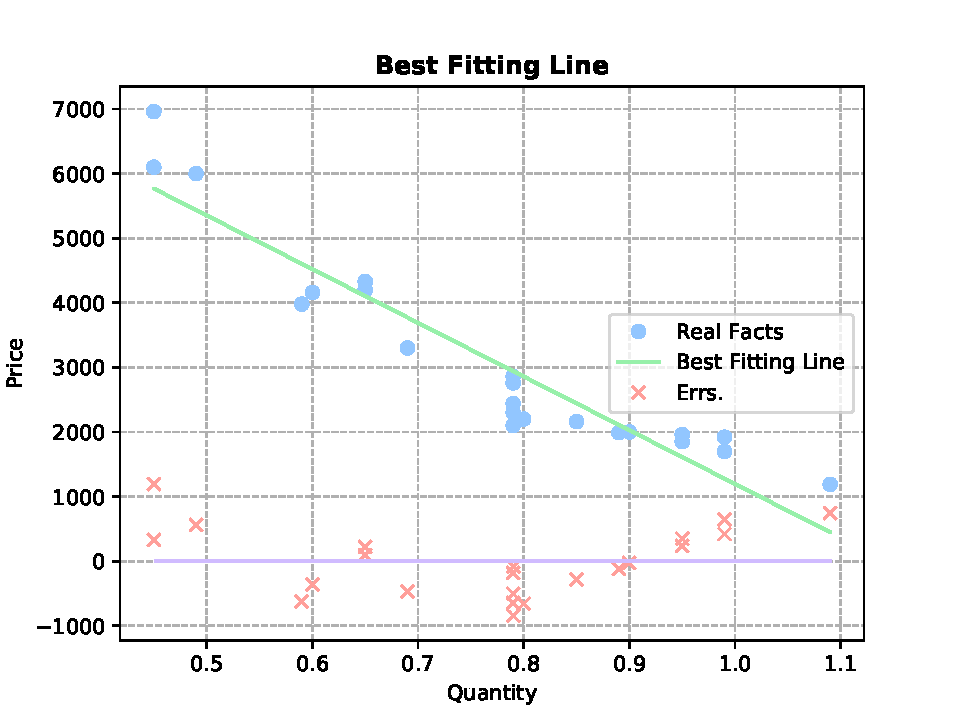
\includegraphics[scale=0.5]{../Graph_2.pdf}
		\caption{Quantity in relation to prices and errors.}
		\label{image2}
	\end{figure}
	The approximated demand curve is enough to make fast decisions and to give a rough idea of how does the market moves with different prices but it's not recommended to use it alone for predictions, still more data is needed.
		
	\subsection{Maximizing with Unitary Cost}
	Now, given the unitary cost of $\$0.23$, it necessary to optimize the function through maximizing its profits (by playing with the different prices in the demand curve). To do this we first need to multiply our demand curve as follows:
		\begin{equation}
			y = (9510.096 -813.3645p)(p-0.23)
			\label{Exercise Two Equation Multiplication}
		\end{equation}
	Then it needs to be differentiated and needs to be solved for p to find its roots and thus maximizing the function as shown in:
		\begin{center}
			\inputminted[
			firstline=171, 
			lastline=175,
			linenos,
			xleftmargin=20pt,
			breaklines, 
			breakautoindent=false,
			] {python}{../src/lab.py}
		\end{center}
	The derivative of the function (\ref{Exercise Two Equation Multiplication}) is:
		\begin{equation}
			y = 11422.403-16628.73p
		\end{equation}
	Thus it follows that \texttt{solve} has a value of 0.687 which means that the company could raise its price to a maximum of $\$ 0.687$ to optimize its profits.
	
	
	

		
		
	
	
	\section*{Acknowledgment}
		I want to personally thank my Differential, Integral and Multivariate Calculus, and now Linear Algebra professor, Christiaan F. J. Ketelaar for not only for inspiring me but for encouraging me every day to give more of myself and for turning the classes into more dynamic ones with subjects of interest to someone who is studying computer science.  I also want to give thanks to my parents for always supporting me through everything and for encouraging me through everything. Last but not least I want to thank God for giving me the opportunity of studying where I am in Guatemala and giving me the strength and wisdom to code everything that needed to be code.
	
%	\section*{References}
%	
%	Please number citations consecutively within brackets \cite{b1}. The 
%	sentence punctuation follows the bracket \cite{b2}. Refer simply to the reference 
%	number, as in \cite{b3}---do not use ``Ref. \cite{b3}'' or ``reference \cite{b3}'' except at 
%	the beginning of a sentence: ``Reference \cite{b3} was the first $\ldots$''
%	
%	Number footnotes separately in superscripts. Place the actual footnote at 
%	the bottom of the column in which it was cited. Do not put footnotes in the 
%	abstract or reference list. Use letters for table footnotes.
%	
%	Unless there are six authors or more give all authors' names; do not use 
%	``et al.''. Papers that have not been published, even if they have been 
%	submitted for publication, should be cited as ``unpublished'' \cite{b4}. Papers 
%	that have been accepted for publication should be cited as ``in press'' \cite{b5}. 
%	Capitalize only the first word in a paper title, except for proper nouns and 
%	element symbols.
%	
%	For papers published in translation journals, please give the English 
%	citation first, followed by the original foreign-language citation \cite{b6}.
%	
%	\begin{thebibliography}{00}
%		\bibitem{b1} G. Eason, B. Noble, and I. N. Sneddon, ``On certain integrals of Lipschitz-Hankel type involving products of Bessel functions,'' Phil. Trans. Roy. Soc. London, vol. A247, pp. 529--551, April 1955.
%		\bibitem{b2} J. Clerk Maxwell, A Treatise on Electricity and Magnetism, 3rd ed., vol. 2. Oxford: Clarendon, 1892, pp.68--73.
%		\bibitem{b3} I. S. Jacobs and C. P. Bean, ``Fine particles, thin films and exchange anisotropy,'' in Magnetism, vol. III, G. T. Rado and H. Suhl, Eds. New York: Academic, 1963, pp. 271--350.
%		\bibitem{b4} K. Elissa, ``Title of paper if known,'' unpublished.
%		\bibitem{b5} R. Nicole, ``Title of paper with only first word capitalized,'' J. Name Stand. Abbrev., in press.
%		\bibitem{b6} Y. Yorozu, M. Hirano, K. Oka, and Y. Tagawa, ``Electron spectroscopy studies on magneto-optical media and plastic substrate interface,'' IEEE Transl. J. Magn. Japan, vol. 2, pp. 740--741, August 1987 [Digests 9th Annual Conf. Magnetics Japan, p. 301, 1982].
%		\bibitem{b7} M. Young, The Technical Writer's Handbook. Mill Valley, CA: University Science, 1989.
%	\end{thebibliography}
%	\vspace{12pt}
%	\color{red}
%	IEEE conference templates contain guidance text for composing and formatting conference papers. Please ensure that all template text is removed from your conference paper prior to submission to the conference. Failure to remove the template text from your paper may result in your paper not being published.
	
\end{document}
